% Name: IOIs ("Items of Interest")
% Description Presentation with periodical updates about dissertation work
% at the Medizinische Hochschule Hannover.
% Author: Bruno Luna
% Date (start): 05.06.2021
% Note: Current PDF version to be sent periodically (objective: weekly)
% to supervisors.

\documentclass[%
	final, %
	% draft, % Grafische Elemente durch graue Boxen ersetzen (beschleunigt Kompilieren)
	% 8pt, % Zu klein, erfordert Paket extsize
	% 9pt, % Zu klein, erfordert Paket extsize
	% 10pt, % für Folien mit sehr viel Text
	11pt, % Standardschriftgröße
	% 12pt, % etwas größer und daher besser zu lesen
	% 14pt, % deutlich größer, erfordert Paket extsize
	% 17pt, % PowerPoint Standardschriftgröße, erfordert Paket extsize
	% 20pt, % sehr groß, erfordert Paket extsize
	% trans,% Zum Erstellen von Overhead Folien
	% handout, % Erstellen eines Handouts
	% article,% Erstellen eines Artikels
 	% compress, % Die Navigation in der Kopfzeile wird komprimiert dargestellt
	t, % Place text of slides at the (vertical) top of the slides
	% c, % Place text of slides at the (vertical) center of the slides
	% color={}, % list of options for color
	xcolor={table,dvipsnames}, % Optionen für xcolor übergeben
	% hyperref={}, % list of options for hyperref
	% envcountsect, % Causes theorems, definitions, and so on to be numbered locally to each section.
	% notheorems, % Switches off the definition of default blocks like theorem
	% noamsthm, % Does not load amsthm and also not amsmath
	% ucs, % lädt ucs Paket
	% utf8, % lädt utf8x Paket von ucs (utf8 enconding)
	% dvips, % erzwingt das Laden des dvips Treibers - idR nicht nötig!
	% usepdftitle=false, % Suppresses the automatic generation of title and author entries in the pdf document information.
	% ignorenonframetext, % suppresses content created for the article mode ??
	show notes, % enables Notes
	% leqno,
	% fleqn,
]{beamer}[2007/03/11] % Minimum necessary version due to severe bugs in version 3.06 !!!

% ~~~~~~~~~~~~~~~~~~~~~~~~~~~~~~~~~~~~~~~~~~~~~~~~~~~~~~~~~~~~~~~~~~~~~~~~
% Fonts Fonts Fonts
% ~~~~~~~~~~~~~~~~~~~~~~~~~~~~~~~~~~~~~~~~~~~~~~~~~~~~~~~~~~~~~~~~~~~~~~~~
\usepackage[T1]{fontenc} % T1 Schrift Encoding
\usepackage{textcomp}	 % additional symbols (Text Companion font extension)


% \usepackage{lmodern}               %% --- Latin Modern
\usepackage{mathptmx}              %% --- Times mit Matheschriften
% \usepackage{mathpazo}              %% --- Palantino
% \usepackage{charter}               %% --- Charter
% \usepackage{bookman}               %% Bookman (lädt Avant Garde !!)
% \usepackage{newcent}               %% New Century Schoolbook (lädt Avant Garde !!)

% \usepackage{bera}
\usepackage[scaled=.90]{helvet}    %% --- Helvetica (Arial)
% \usepackage{cmbright}              %% --- CM-Bright (eigntlich eine Familie)
% \usepackage{tpslifonts}            %% --- (Font for Slides)
% \usepackage{avant}      	          %% --- Avantgard
%
\usepackage{courier}               %% --- Courier
%\usepackage[scaled=0.9]{luximono}  	 %% --- Luxi Mono


%%% ===== Sans Serif (kommerzielle Schriften) ============================

% \usepackage[scaled=0.90]{frutiger}  %% --- Adobe Frutiger
% \usepackage[scaled=0.94]{futura}    %% --- Adobe Futura (=Linotype FuturaLT) : Sans Serif
% \usepackage{gillsans}               %% --- Adobe Gill Sans : Sans Serif
% \renewcommand{\sfdefault}{pmy}      %% -- Adobe Myriad  : Sans Serif
% \usepackage[scaled]{asyntax}        %% --- Syntax : sans serif font
% \usepackage[medium]{optima}         %% --- Adobe Optima : Semi Sans Serif
% \renewcommand{\sfdefault}{lo9}      %% --- Linotype ITC Officina Sans

%% ===== Serifen (kommerzielle Schriften ) ================================

% \renewcommand{\rmdefault}{pasx}     %% --- Adobe Aldus
% \usepackage[scaled=1.05]{xagaramon} %% --- Adobe Garamond
% \renewcommand{\rmdefault}{pegx}     %% --- Adobe Stempel Garamond
% \renewcommand{\rmdefault}{pml}      %% --- Adobe Melior
% \renewcommand{\rmdefault}{pmnx}     %% --- Adobe Minion
% \renewcommand{\rmdefault}{psbx}     %% --- Adobe Sabon
% \renewcommand{\rmdefault}{lch}      %% --- Linotype ITC Charter
% \renewcommand{\rmdefault}{lmd}      %% --- Linotype Meridien

% *** Sprache *****************************
\usepackage[english]{babel}
\usepackage[latin1]{inputenc}
%------------------------------------------

% Define date
%\usepackage{datetime}

%%% Doc: ftp://tug.ctan.org/pub/tex-archive/macros/latex/required/graphics/grfguide.pdf
% Bilder
\usepackage[%
   %final,
   %draft % do not include images (faster)
]{graphicx}



%%% Emulationspakete
% \usepackage{beamerprosper}
% \usepackage{beamerseminar}
% \usepackage{beamerfoils}
% \usepackage{beamertexpower}


%%% 4.6.2    Printing the Handout
% \usepackage{pgfpages}
% \pgfpagelayout{resize}[a4paper,border shrink=5mm,landscape]
%     This says “Resize all pages to landscape A4 pages, no what their original size was, but shrink the pages
% by 5mm, so that there is a bit of a border around everything.” Naturally, instead of a4paper you can also use
% letterpaper or any of the other standard paper sizes. For further options and details see the documentation
% of pgfpages.
% \pgfpagelayout{2 on 1}[a4paper,border shrink=5mm]


% \usepackage{multimedia}
%     A stand-alone package that implements several commands for including external animation and sound
%     files in a pdf document. The package can be used together with both dvips plus ps2pdf and pdflatex,
%     though the special sound support is available only in pdflatex.



%% sonstige Pakete ========================
%
% \usepackage{enumitem}
% \usepackage{units}
% \usepackage{pifont}
% \usepackage{subscript}
% -----------------------------------------

\usepackage{tabularx}   % Erweiterte Tabellen Optionen
\usepackage{booktabs}
\usepackage{multicol}
\usepackage{url}






% *****************************************
% >>> Themes <<<<<<<<<<<<<<<<<<<<<<<<<<<<<<
% *****************************************

% \usetheme[<options>]{<name list>} 		Installs the presentation theme named <name>.
% \usecolortheme[<options>]{<name list>} Same as \usetheme, only for color themes.
% \usefonttheme[<options>]{<name>} 		Same as \usetheme, only for font themes.
% \useinnertheme[<options>]{<name>}		Same as \usetheme, only for inner themes.
% \useoutertheme[<options>]{<name>}		Same as \usetheme, only for outer themes.

% *****************************************
% >>> Themes ohne Navigation
% *****************************************
% \usetheme{default}
% -------------------------------
% \usetheme[]{Bergen}
% -------------------------------
% \usetheme[%
% 	secheader % section im Header
% ]{Boadilla}
% -------------------------------
% % Wie das Boadilla theme, mit kraeftigeren Farben
% % und unveraenderten Icons
% \usetheme[%
% 	secheader % section im Header
% ]{Madrid}
% -------------------------------
% \usetheme{Pittsburgh}
% -------------------------------
% \usetheme[]{Rochester}


% *****************************************
% >>> Themes mit Navigation (Baumstruktur)
% *****************************************
% \usetheme{Antibes}      % flach
% -------------------------------
% \usetheme{JuanLesPins}  % 3D, Schatten
% -------------------------------
% \usetheme{Montpellier}    % flach, wenig Farben


% *****************************************
% >>> Themes mit Navigation (Sidebar)
% *****************************************
% % flach, starke Farben
% \usetheme[%
%  	left, % sidebar links
% % 	right, % sidebar rechts
% % 	hideallsubsections, % nur sections werden angezeigt
% % 	hideothersubsections, % nur subsections der aktuellen section werden angezeigt
% ]{Berkeley}
% -------------------------------
% % wie Berkeley, 3D, starke Farben
% \usetheme[%
%  	left, % sidebar links
% % 	right, % sidebar rechts
% % 	hideallsubsections, % nur sections werden angezeigt
% % 	hideothersubsections, % nur subsections der aktuellen section werden angezeigt
% ]{PaloAlto}
% -------------------------------
% % flach, schwache Farben
% \usetheme[%
%  	left, % sidebar links
% % 	right, % sidebar rechts
% % 	hideallsubsections, % nur sections werden angezeigt
% % 	hideothersubsections, % nur subsections der aktuellen section werden angezeigt
% ]{Goettingen}
% -------------------------------
% % wie Goettingen, flach, starke Farben
% \usetheme[%
%  	left, % sidebar links
% % 	right, % sidebar rechts
% % 	hideallsubsections, % nur sections werden angezeigt
% % 	hideothersubsections, % nur subsections der aktuellen section werden angezeigt
% ]{Marburg}
% -------------------------------
% flach, schwache Farben
% \usetheme[%
% % 	hideallsubsections, % nur sections werden angezeigt
% % 	hideothersubsections, % nur subsections der aktuellen section werden angezeigt
% ]{Hannover}


% *****************************************
% >>> Themes mit Navigation (Mini Frame Navigation)
% *****************************************
% % starke Farben, flach
% \usetheme[
% % 	compress, % Navigation in einer Zeile
% ]{Berlin}
% -------------------------------
% % wie Berlin, runde Kanten, starke Farben, flach
% \usetheme[
% 	compress, % Navigation in einer Zeile
% ]{Ilmenau}
% -------------------------------
% % wie Berlin, starke Farben, flach
% \usetheme[
% 	compress, % Navigation in einer Zeile
% ]{Dresden}
% -------------------------------
% % starke Farben, 3D
% \usetheme{Darmstadt}
% -------------------------------
% % wie Darmstadt, ohne subsections
% \usetheme{Frankfurt}
% -------------------------------
% % flach, schwache Farben
% \usetheme{Singapore}
% -------------------------------
% % flach, horiz. Linien
% \usetheme{Szeged}


% *****************************************
% >>> Themes mit Navigation (Section and Subsection Tables)
% *****************************************
% % flach, rund, starke Farben
% \usetheme{Copenhagen}
% -------------------------------
% % flach, eckig, starke Farben
% \usetheme{Luebeck}
% -------------------------------
% % flach, starke Farben
% \usetheme{Malmoe}
% -------------------------------
% 3D, starke Farben
\usetheme{Warsaw}


% *****************************************
% >>>> 15.1    Inner Themes
% *****************************************
% An inner theme installs templates that dictate how the following elements are typeset:
%    - Title and part pages.
%    - Itemize environments.
%    - Enumerate environments.
%    - Description environments.
%    - Block environments.
%    - Theorem and proof environments.
%    - Figures and tables.
%    - Footnotes.
%    - Bibliography entries.


% >>>  Itemize Bullets
% -------------------------------
% \useinnertheme{default} % Zahlen
% -------------------------------
% \useinnertheme{circles} % Kreise
% -------------------------------
\useinnertheme{rectangles} % Vierecke
% -------------------------------
% \useinnertheme[%
% 	shadow % mit Schatten
% ]{rounded} % 3D Kugeln
% -------------------------------
% \useinnertheme{inmargin} % Bullts im Margin


% *****************************************
% >>>> 15.2    Outer Themes
% *****************************************
% An outer theme dictates (roughly) the overall layout of frames. It specifies where any navigational elements
% should go (like a mini table of contents or navigational mini frames) and what they should look like. Typically,
% an outer theme specifies how the following elements are rendered:
%    - The head- and footline.
%    - The sidebars.
%    - The logo.
%    - The frame title.

% \useoutertheme{default}
% -------------------------------
% \useoutertheme{infolines}
% -------------------------------
% \useoutertheme[%
% 	footline=empty, % suppressed the footline (default).
% % 	footline=authorinstitute, %shows the author's name and the institute in the footline.
% % 	footline=authortitle, % shows the author's name and the title in the footline.
% % 	footline=institutetitle, % shows the institute and the title in the footline.
% % 	footline=authorinstitutetitle, % shows the author's name, the institute, and the title in the footline.

% ]{miniframes}
% -------------------------------
% \useoutertheme[%
% % 	subsection= true,  % or false shows or suppresses line showing the subsection in the headline.
% ]{smoothbars}
% -------------------------------
% \useoutertheme[%
%  	left, % sidebar links
% % 	right, % sidebar rechts
% % 	hideallsubsections, % nur sections werden angezeigt
% % 	hideothersubsections, % nur subsections der aktuellen section werden angezeigt
% ]{sidebar}
% -------------------------------
% % This theme installs a headline in which, on the left, the sections of the talk are shown and, on the right,
% % the subsections of the current section. If the class option compress has been given, the sections and
% % subsections will be put in one line; normally there is one line per section or subsection.
% \useoutertheme{split}
% The colors are taken from palette primary and palette fourth.
% -------------------------------
% % This layout theme extends the split theme by putting a horizontal shading behind the frame title and
% % adding a little 'shadow' at the bottom of the headline.
% \useoutertheme{shadow}
% -------------------------------
% \useoutertheme[
% % 	hooks, % Einruecken der Abschnittsueberschriften in der Kopfzeile
% ]{tree}
% -------------------------------
% wie tree, ohne die Linien
% \useoutertheme{smoothtree}


% *****************************************
% >>>> 16.1    Color Themes
% *****************************************
% \usecolortheme{default}
% \usecolortheme{structure}
% \usecolortheme{sidebartab}

% *****************************************
% >>>> 16.1.2    Complete Color Themes
% A 'complete' color theme is a color theme that completely specifies all colors for all parts of a frame. It
% installs specific colors and does not derive the colors from, say, the structure beamer-color. Complete
% color themes happen to have names of flying animals.

% -------------------------------
% \usecolortheme{default}
% -------------------------------
\usecolortheme[%
% 	named=red,
% 	named=blue,
% 	named=green,
% 	named=orange,
% 	named=gray,
 	named=NavyBlue,
%  named=RoyalBlue,
%  named=MidnightBlue,
%  named=CadetBlue,
]{structure}
% Farben aus dvipsnam.def: (Option 'dvipsnames' fuer xcolor muss geladen sein!)
% http://www.math.utu.fi/opetusohj/latex/doc/palette.pdf
% GreenYellow, Yellow, Goldenrod, Dandelion, Apricot, Peach, Melon, YellowOrange, Orange, BurntOrange, Bittersweet, RedOrange, Mahogany, Maroon, BrickRed, Red, OrangeRed, RubineRed, WildStrawberry, Salmon, CarnationPink, Magenta, VioletRed, Rhodamine, Mulberry, RedViolet, Fuchsia, Lavender, , Thistle, Orchid, DarkOrchid, Purple, Plum, Violet, RoyalPurple, BlueViolet, Periwinkle, CadetBlue, CornflowerBlue, MidnightBlue, NavyBlue, RoyalBlue, Blue, Cerulean, Cyan, ProcessBlue, , SkyBlue, Turquoise, TealBlue, Aquamarine, BlueGreen, Emerald, JungleGreen, SeaGreen, Greenv,  ForestGreen, PineGreen, LimeGreen, YellowGreen, SpringGreen, OliveGreen, RawSienna, Sepia, Brown, Tan, Gray, Black, White
% -------------------------------
% % blau-schwarz, Hintergrund: blau
% \usecolortheme[%
% %  	overlystylish
% ]{albatross}
% -------------------------------
% % blau-schwarz, Hintergrund: weiss
% \usecolortheme{lily}
% -------------------------------
% % blau-grau, , Hintergrund: grau
% \usecolortheme{beetle}
% -------------------------------
% % gelb-weiss, , Hintergrund: weiss
% \usecolortheme{crane}
% -------------------------------
% grau-grau (hell)
% \usecolortheme{dove}
% -------------------------------
% % grau-grau (dunkel)
% \usecolortheme{fly}
% -------------------------------
% % grau-grau-weiss (hell) mit Boxen
% \usecolortheme{seagull}
% -------------------------------
% % gelb-orange-grau
% \usecolortheme{wolverine}
% -------------------------------
% % grau
% \usecolortheme{beaver}

% *****************************************
% >>>> 16.1.3    Inner Color Themes
% Inner color themes only specify the colors of elements used in inner themes. Most noticably, they specify
% the colors used for blocks. They can be used together with other (color) themes. If they are used to change
% the inner colors installed by a presentation theme or another color theme, they should obviously be specified
% after the other theme has been loaded. Inner color themes happen to have fl�ower names.
% -------------------------------
% \usecolortheme{lily} % keine Boxen
% -------------------------------
% \usecolortheme{orchid} % Boxen mit starken Farben
% -------------------------------
% \usecolortheme{rose} % Boxen mit schwachen Farben

% *****************************************
% >>>> 16.1.4    Outer Color Themes
% An outer color theme changes the palette colors, on which the colors used in the headline, footline, and
% sidebar are based by default. Outer color themes normally do not change the color of inner elements, except
% possibly for titlelike. They have happen to sea-animal names.

% -------------------------------
% % Titel mit Farbe, starke Farben
% \usecolortheme{whale}
% -------------------------------
% % Titel mit Farbe, schwache Farben
% \usecolortheme{seahorse}
% -------------------------------
% % Titel ohne Farbe, starke Farben
% \usecolortheme{dolphin}

% *****************************************
% Detailierte Veraenderungen der Farben
% *****************************************
% \setbeamercolor*{author in head/foot}{parent=palette tertiary}
% \setbeamercolor*{title in head/foot}{parent=palette secondary}
% \setbeamercolor*{date in head/foot}{parent=palette primary}
% \setbeamercolor*{section in head/foot}{parent=palette secondary} %tertiary
% \setbeamercolor*{subsection in head/foot}{parent=palette primary}
% Elemente deren Farbe veraendert werden kann
% \setbeamercolor{normal text}{fg=black}
% \setbeamercolor*{example text}
% \setbeamercolor*{titlelike}
% \setbeamercolor*{separation line}
% \setbeamercolor*{upper separation line head}
% \setbeamercolor*{separation line}
% \setbeamercolor*{middle separation line head}
% \setbeamercolor*{separation line}
% \setbeamercolor*{lower separation line head}
% \setbeamercolor*{upper separation line foot}
% \setbeamercolor*{middle separation line foot}
% \setbeamercolor*{lower separation line foot}
% -------------------------------
% \setbeamercolor*{math text}
% \setbeamercolor*{math text inlined}
% \setbeamercolor*{math text displayed}
% \setbeamercolor*{normal text in math text}
% -------------------------------
% Nutzung:
% \usebeamercolor[fg]{normal text}
% \setbeamercolor{normal text}{fg=black,bg=mylightgrey}
% -------------------------------
% Palette:
% \setbeamercolor{palette primary}
% \setbeamercolor{palette secondary}
% \setbeamercolor{palette tertiary}
% \setbeamercolor{palette quaternary}
% -------------------------------
% \setbeamercolor{palette sidebar primary}
% \setbeamercolor{palette sidebar secondary}
% \setbeamercolor{palette sidebar tertiary}
% \setbeamercolor{palette sidebar quaternary}




% *****************************************
% Transparenz Effekte
% *****************************************

\setbeamercovered{invisible} % is the default and causes covered text to 'completely disappear.
% \setbeamercovered{transparent} % Durchscheinen des Textes
% \setbeamercovered{dynamic} % Einblenden
% \setbeamercovered{highly dynamic} % Einblenden


% *****************************************
% >>>> 17.1 Font Themes
% *****************************************
% \usefonttheme{default}
% The default font theme installs a sans serif font for all text of the presentation. The default theme
% installs different font sizes for things like titles or head- and footlines, but does not use boldface or
% italics for 'hilighting.' To change some or all text to a serif font, use the serif theme.
% -------------------------------
% \usefonttheme{professionalfonts}
% This font theme does not really change any fonts. Rather, it suppresses certain internal replacements
% performed by beamer. If you use 'professional fonts' (fonts that you buy and that come with a
% complete set of every symbol in all modes), you do not want beamer to meddle with the fonts you use.
% -------------------------------
% \usefonttheme[%
% % 	stillsansserifmath, % mathematical text typeset using sans serif.
% % 	stillsansserifsmall, % will cause 'small' text to be still typeset using sans serif. This refers to
%  								% the text in the headline, footline, and sidebars. Using this options is often
%  								% advisable since small  text is often easier to read in sans serif.
% % 	stillsansseriflarge, %  Titel still   typeset using sans serif
% %  	onlymath, % typset math in serif but nothing else
% ]{serif}
% -------------------------------
% \usefonttheme[%
% % 	onlysmall, % headline, footline, and sidebars is changed
% % 	onlylarge, % main title, frame titles, and section
% ]{structurebold}
% -------------------------------
% \usefonttheme[%
% % 	onlysmall, % headline, footline, and sidebars is changed
% % 	onlylarge, % main title, frame titles, and section
% ]{structureitalicserif}
% -------------------------------
% \usefonttheme[%
% % 	onlysmall, % headline, footline, and sidebars is changed
% % 	onlylarge, % main title, frame titles, and section
% ]{structuresmallcapsserif}



% *****************************************
% >>>> Veraendern der Schrifteinstellung definierter Elemente
% *****************************************

% Beispiele
% \setbeamerfont{frametitle}{size=\large}
% \setbeamerfont{frametitle}{series=\bfseries}

% weitere Befehle
% size= size command sets the size attribute of the beamerfont.
% size*={ size in pt }{ baselineskip }
% shape= (\itshape, \slshape, \scshape, or \upshape)
% series= (command like \bfseries.)
% family= (command like \rmfamily or \sffamily).
% family*={ family name } (For example, the family name for Times happens to be ptm. )
% parent={ parent list } specifies a list of parent fonts.
%
% Example for parent
% \setbeamerfont{parent A}{size=\large}
% \setbeamerfont{parent B}{series=\bfseries}
% \setbeamerfont{child}{parent={parent A, parent B},size=\small}
%
% \usebeamerfont{child}
% This text is small and bold.

% *****************************************
% >>>> 15.3.2    Using Beamer's Templates
% *****************************************
% As a user of the beamer class you typically do not 'use' or 'invoke' templates yourself, directly. For
% example, the frame title template is automatically invoked by beamer somewhere deep inside the frame
% typesetting process. The same is true of most other templates. However, if, for whatever reason, you wish
% to invoke a template yourself, you can use the following command.
% \usebeamertemplate***{ element name }
% -------------------------------
%%% 7.2.1 The Headline and Footline
% \setbeamertemplate{headline} % Beamer-Template/-Color/-Font
% \setbeamertemplate{headline}
% {%
%   \begin{beamercolorbox}{section in head/foot}
%     \vskip2pt\insertnavigation{\paperwidth}\vskip2pt
%   \end{beamercolorbox}%
% }
% \setbeamertemplate{headline}[default] % The default is just an empty headline.
% \setbeamertemplate{headline}[infolines theme]
% \setbeamertemplate{headline}[miniframes theme]
% \setbeamertemplate{headline}[sidebar theme]
% \setbeamertemplate{headline}[smoothtree theme]
% \setbeamertemplate{headline}[smoothbars theme]
% \setbeamertemplate{headline}[tree]
% \setbeamertemplate{headline}[split theme]
% \setbeamertemplate{headline}[text line]{ text } % The headline is typeset with 'text'
% -------------------------------
% \setbeamertemplate{footline} % Beamer-Template/-Color/-Font
% \setbeamertemplate{footline}[default]
% \setbeamertemplate{footline}[infolines theme]
% \setbeamertemplate{footline}[miniframes theme]
% \setbeamertemplate{footline}[page number]
% \setbeamertemplate{footline}[frame number]
% \setbeamertemplate{footline}[split]
% \setbeamertemplate{footline}[text line]{ text }
% -------------------------------
%%% 7.2.2 The Sidebars
% -------------------------------
%%% 7.2.3 Navigation Bars (funktioniert nur mit miniframe Themes)
% \setbeamertemplate{mini frames}[default] % shows small circles as mini frames.
\setbeamertemplate{mini frames}[box] % shows small rectangles as mini frames.
% \setbeamertemplate{mini frames}[tick] % shows small vertical bars as mini frames.
% -------------------------------
%%% 7.2.4 The Navigation Symbols
%%% Beamer-Template/-Color/-Font navigation symbols
\setbeamertemplate{navigation symbols}{} % suppresses all navigation symbols:
% \setbeamertemplate{navigation symbols}[horizontal] % Organizes the navigation symbols horizontally.
% \setbeamertemplate{navigation symbols}[vertical] % Organizes the navigation symbols vertically.
% \setbeamertemplate{navigation symbols}[only frame symbol] % Shows only the navigational symbol for navigating frames.
% -------------------------------
%%% 7.2.5 The Logo
% \setbeamertemplate{logo} % Beamer-Template/-Color/-Font
% -------------------------------
%%% 7.2.6 The Frame Title
% \setbeamertemplate{frametitle} % Beamer-Template/-Color/-Font
% \setbeamertemplate{frametitle}[default][left] % left, center, right
% \setbeamertemplate{frametitle}[shadow theme]
% \setbeamertemplate{frametitle}[sidebar theme]
% \setbeamertemplate{frametitle}[smoothbars theme]
% \setbeamertemplate{frametitle}[smoothtree theme]
% -------------------------------
%%% 7.2.7 The Background
% \setbeamertemplate{background canvas} % Beamer-Template/-Color/-Font
% \setbeamertemplate{background canvas}[default]
% \setbeamertemplate{background canvas}[vertical shading][ color options ] installs a vertically shaded background.
%     - top= color specifies the color at the top of the page. By default, 25% of the foreground of
%       the beamer-color palette primary is used.
%     - bottom= color specifies the color at the bottom of the page. By default, the background of
%       normal text at the moment of invocation of this command is used.
%     - middle= color specifies the color for the middle of the page. Thus, if this option is given, the
%       shading changes from the bottom color to this color and then to the top color.
%     - midpoint= factor specifies at which point of the page the middle color is used. A factor of 0
%       is the bottom of the page, a factor of 1 is the top. The default, which is 0.5 is in the middle.
% \setbeamertemplate{background} % Beamer-Template/-Color/-Font
% \setbeamertemplate{background}[default] % is empty.
% \setbeamertemplate{background}[grid][step=1cm] % places a grid on the background.
%     - step= dimension specifies the distance between grid lines. The default is 0.5cm.
%     - color= color specifies the color of the grid lines. The default is 10% foreground.
% -------------------------------
%%% 7.3 Margin Sizes
\setbeamersize{text margin left=2em,text margin right=2em}
% \setbeamersize{sidebar width left=2cm}
%         - text margin left= TEX dimension sets a new left margin. This excludes the left sidebar. Thus,
%           it is the distance between the right edge of the left sidebar and the left edge of the text.
%         - text margin right= TEX dimension sets a new right margin.
%         - sidebar width left= TEX dimension sets the size of the left sidebar. Currently, this command
%           should be given before a shading is installed for the sidebar canvas.
%         - sidebar width right= TEX dimension sets the size of the right sidebar.
%         - description width= TEX dimension sets the default width of description labels, see Section 11.1.
%         - description width of= text sets the default width of description labels to the width of the
%             text , see Section 11.1.
%         - mini frame size= TEX dimension sets the size of mini frames in a navigation bar. When two
%           mini frame icons are shown alongside each other, their left end points are TEX dimension far
%           apart.
%         - mini frame offset= TEX dimension set an additional vertical offset that is added to the mini
%           frame size when arranging mini frames vertically.
% -------------------------------
%%% 9.1 Adding a Title Page
% \setbeamersize{title page} % Beamer-Template/-Color/-Font
%    This template is invoked when the \titlepage command is used.
%    The following commands are useful for this template:
%     -  \insertauthor inserts a version of the author's name that is useful for the title page.
%     -  \insertdate inserts the date.
%     -  \insertinstitute inserts the institute.
%     -  \inserttitle inserts a version of the document title that is useful for the title page.
%     -  \insertsubtitle inserts a version of the document title that is useful for the title page.
%     -  \inserttitlegraphic inserts the title graphic into a template.
% -------------------------------
%%% 9.2 Adding Sections and Subsections
% -------------------------------
%%% Parent Beamer-Template sections/subsections in toc
% This is a parent template, whose children are section in toc and subsection in toc.
% \setbeamertemplate{sections/subsections in toc}[default]
% \setbeamertemplate{sections/subsections in toc}[sections numbered]
% \setbeamertemplate{sections/subsections in toc}[subsections numbered]
% \setbeamertemplate{sections/subsections in toc}[circle]
\setbeamertemplate{sections/subsections in toc}[square]
% \setbeamertemplate{sections/subsections in toc}[ball]
% \setbeamertemplate{sections/subsections in toc}[ball unnumbered]
% -------------------------------
%%% 9.6 Adding a Bibliography
% -------------------------------
% \setbeamertemplate{bibliography item} % Beamer-Template/-Color/-Font
\setbeamertemplate{bibliography item}[default] %  little article icon as the reference
% \setbeamertemplate{bibliography item}[article] % Alias for the default.
% \setbeamertemplate{bibliography item}[book] % little book icon as the reference
% \setbeamertemplate{bibliography item}[triangle] % triangle as the reference
% \setbeamertemplate{bibliography item}[text] % reference text (like '[Dijkstra, 1982]')
% -------------------------------
%%% 10.1 Adding Hyperlinks and Buttons
% -------------------------------
%%% 11.1 Itemizations, Enumerations, and Descriptions
% \setbeamertemplate{items} % parent template of itemize items and enumerate items
% \setbeamertemplate{itemize items} % Parent Beamer-Template
\setbeamertemplate{itemize items}[triangle]
% \setbeamertemplate{itemize items}[circle]
% \setbeamertemplate{itemize items}[square]
% \setbeamertemplate{itemize items}[ball]
% -------------------------------
% \setbeamertemplate{enumerate items}[default] % Numbered
% \setbeamertemplate{enumerate items}[circle] % Places the numbers inside little circles.
\setbeamertemplate{enumerate items}[square] % Places the numbers on little squares.
% \setbeamertemplate{enumerate items}[ball] % 'Projects' the numbers onto little balls.
% -------------------------------
%%% 11.2 Hilighting
% -------------------------------
%%% 11.3 Block Environments
% \setbeamertemplate{blocks} % Parent Beamer-Template
% \setbeamertemplate{blocks}[default]
\setbeamertemplate{blocks}[rounded][shadow=true]
% \setbeamertemplate{blocks}[rounded][shadow=false]
% -------------------------------
%%% 11.4 Theorem Environments
% \setbeamertemplate{qed symbol} % Beamer-Template/-Color/-Font
% -------------------------------
% \setbeamertemplate{theorems} % Parent Beamer-Template
% \setbeamertemplate{theorems}[default]
% \setbeamertemplate{theorems}[normal font]
% \setbeamertemplate{theorems}[numbered]
% \setbeamertemplate{theorems}[ams style]
% -------------------------------
%%% 11.6 Figures and Tables
% \setbeamertemplate{caption} % Beamer-Template/-Color/-Font
% \setbeamertemplate{caption}[default] typesets the caption name (a word like 'Figure' or 'Abbildung' or 'Table')
% \setbeamertemplate{caption}[numbered] adds the figure or table number to the caption.
% \setbeamertemplate{caption}[caption name own line]
% -------------------------------
% \setbeamertemplate{caption name} % Beamer-Color/-Font
% -------------------------------
%%% 11.10    Abstract
% -------------------------------
%%% 11.11 Verse, Quotations, Quotes
% -------------------------------
%%% 11.12 Footnotes
% -------------------------------
%%% 18.1 Specifying Note Contents
% \setbeamertemplate{note page} % Beamer-Template/-Color/-Font
% \setbeamertemplate{note page}[default]
% \setbeamertemplate{note page}[compress]
% \setbeamertemplate{note page}[plain]
% -------------------------------
%%% Specifying Which Notes and Frames Are Shown
% \setbeameroption{hide notes}
% \setbeameroption{show notes}
% \setbeameroption{show notes on second screen= location }
% \setbeameroption{show only notes}
%% Eigene Definitionen ============================
%

\newcommand{\therfore}{\ding{225}\mbox{ }}
\newcommand{\verythinarrow}{\ding{221}\mbox{ }}
\newcommand{\thinarrow}{\ding{222}\mbox{ }}
\newcommand{\newarrow}{\ding{222}\mbox{ }}
\newcommand{\addspace}{\vspace{0.5\baselineskip}}



% Providing author name before "begin{document}" to avoid warning
\author{Bruno Luna}

\begin{document}
	\title{Dissertation Project}
\subtitle{Periodical Update}
%\author{Bruno Luna}
\institute{Medizinische Hochschule Hannover}
\titlegraphic{}
%\newdate{date}{05}{06}{2021}
%\date{\displaydate{date}}
\date{\today}
% --------------------------------------------------- Slide --
\begin{frame}[plain]
  \titlepage
\end{frame}
	%% ------------------------------------------------------------
\section{Calendar Week}
% ------------------------------------------------------------
% --------------------------------------------------- Slide --
\subsection{CW 05}
% ------------------------------------------------------------
\begin{frame}
  \frametitle{Review CW 05}
	\begin{itemize}
		\item First presentation of status of work to Dr. Greuling/R. Werth/O.Roffmann at MHH. \textcolor{green}{Done at CW03}
		\item Implementation of first comments (mostly related to formatting/presentation) \textcolor{green}{Done at CW04}
		\item Presentation of status of work for discussion with Prof.Dr. Stiesch and Dr. Greuling (via online meeting). \textcolor{green}{Done}
	\end{itemize}
\end{frame}


% ------------------------------------------------------------
% --------------------------------------------------- Slide --
\subsection{CW 06}
% ------------------------------------------------------------
% ------------------------------------------------------------
\begin{frame}
  \frametitle{Outlook CW 06}
	\begin{itemize}
		\item Proceed with implementation of further comments (related to content).
		\item Set an appointment with O.Roffmann for Ansys-related discussion (Ansys distributed server and scripting in SpaceClaim).
		\item Start reading in more details about bone remodelling. Relevant chapters from "Dental Implant Prosthetics" by C. Misch (2015) as initial reference.
	\end{itemize}
\end{frame}
% --------------------------------------------------- Slide --


	%% ------------------------------------------------------------
\section{Calendar Week}
% ------------------------------------------------------------
% --------------------------------------------------- Slide --
\subsection{CW 06/07}
% ------------------------------------------------------------
\begin{frame}
  \frametitle{Review CW 06/07}
	\begin{itemize}
		\item Finished chapters 1 to 6 of book "Dental Implant Prosthetics" by C. Misch (2015), including introduction to bone remodelling theory (chap.6)  \textcolor{green}{Done}
		\item Installed MS Teams with MHH account with support from IT. Therefore now able to not only take part, but also set own Teams Meetings \textcolor{green}{Done}
		\item Set first meeting with Oliver Roffmann for Ansys discussions. \textcolor{green}{Done}
	\end{itemize}
\end{frame}


% ------------------------------------------------------------
% --------------------------------------------------- Slide --
\subsection{CW 08}
% ------------------------------------------------------------
% ------------------------------------------------------------
\begin{frame}
  \frametitle{Outlook CW 08}
	\begin{itemize}
		\item Discussion with O.Roffmann about Ansys-related topics (Ansys distributed server and scripting in SpaceClaim).
		\item Continue reading in more details about bone remodelling. Start with papers from Frost, which are cited by many other researchers.
	\end{itemize}
\end{frame}
% --------------------------------------------------- Slide --


	%% ------------------------------------------------------------
\section{Calendar Week}
% ------------------------------------------------------------
% --------------------------------------------------- Slide --
\subsection{CW 08}
% ------------------------------------------------------------
\begin{frame}[allowframebreaks]
  \frametitle{Review CW 08}
	\begin{itemize}
		\item Experience and knowledge exchanged with O.Roffmann on 23.02.2022 regarding following Ansys topics: \textcolor{green}{Done}
		\begin{itemize}
		\item Bruno showed the Python Script created for automatization of geometry generation. Also shared a few documents with instructions of how to create such scripts in Python/SpaceClaim.
		\item Oliver showed the topic he is working on (FGM Implants) and how he approached the issue of variation of E-Modul with a "proxy-temperature" dependent material property. It is expected that this might help in diminishing the effects of stress singularity due to the interface of different materials. Very interesting approach that might be useful for our work as well.
		\item Oliver prepared a step-by-step of how to configure the RSM (Remote Solver Manager) for the MHH Ansys computing server.
		\item Bruno prepared a step-by-step of how to use the "Named Selection Worksheet" in Ansys Workbench to select ranges of nodes or elements (question from Oliver regarding Bruno's presentation in January).
		\item General exchange about relevant literature (papers, books, etc.)
		\end{itemize}
		\item Configuration of Ansys RSM performed. First test performed. It worked correctly, so that RSM can be used for future calculations involving more complicated geometries (e.g., reference from Dr. Brune) \textcolor{green}{Done}
		\item Finished chapters 8 of book "Dental Implant Prosthetics" by C. Misch (2015), covering the stress theorem for implant treatment  \textcolor{green}{Done}
	\end{itemize}
\end{frame}


% ------------------------------------------------------------
% --------------------------------------------------- Slide --
\subsection{CW 09}
% ------------------------------------------------------------
% ------------------------------------------------------------
\begin{frame}
  \frametitle{Outlook CW 09}
	\begin{itemize}
		\item Continue reading in more details about bone remodelling. Start with papers from Frost, which are cited by many other researchers.
		\item During search for literature regarding bone remodelling (see above), some free available APDL scripts for education purposes from the University of Ulm and University of Sidney. Start with trying to reproduce the results of the tutorials, as it might be a good lead of how to create our own scripts.
	\end{itemize}
\end{frame}
% --------------------------------------------------- Slide --


	%% ------------------------------------------------------------
\section{Calendar Week}
% ------------------------------------------------------------
% --------------------------------------------------- Slide --
\subsection{CW 09}
% ------------------------------------------------------------
\begin{frame}
  \frametitle{Review CW 09}
	\begin{itemize}
		\item All APDL Script tutorials/exercises regarding remodelling algorithm provided by the University of Ulm were tested. Where possible, results were checked against analytical calculations. \textcolor{green}{Done}
		\item Backup of files in the MHH PC where organized. "Readme" file under \path{\ZPR\2_Forschung\Bereiche\WPL\FEM\BLuna\6_Ansys} now contains a detailed description of how to restore the files. Also the overview of the Ansys files created is available in the the same folder. \textcolor{green}{Done}
	\end{itemize}
\end{frame}

\begin{frame}
  \frametitle{Review CW 09 - First Remodeling Simulations}
	\begin{figure}
		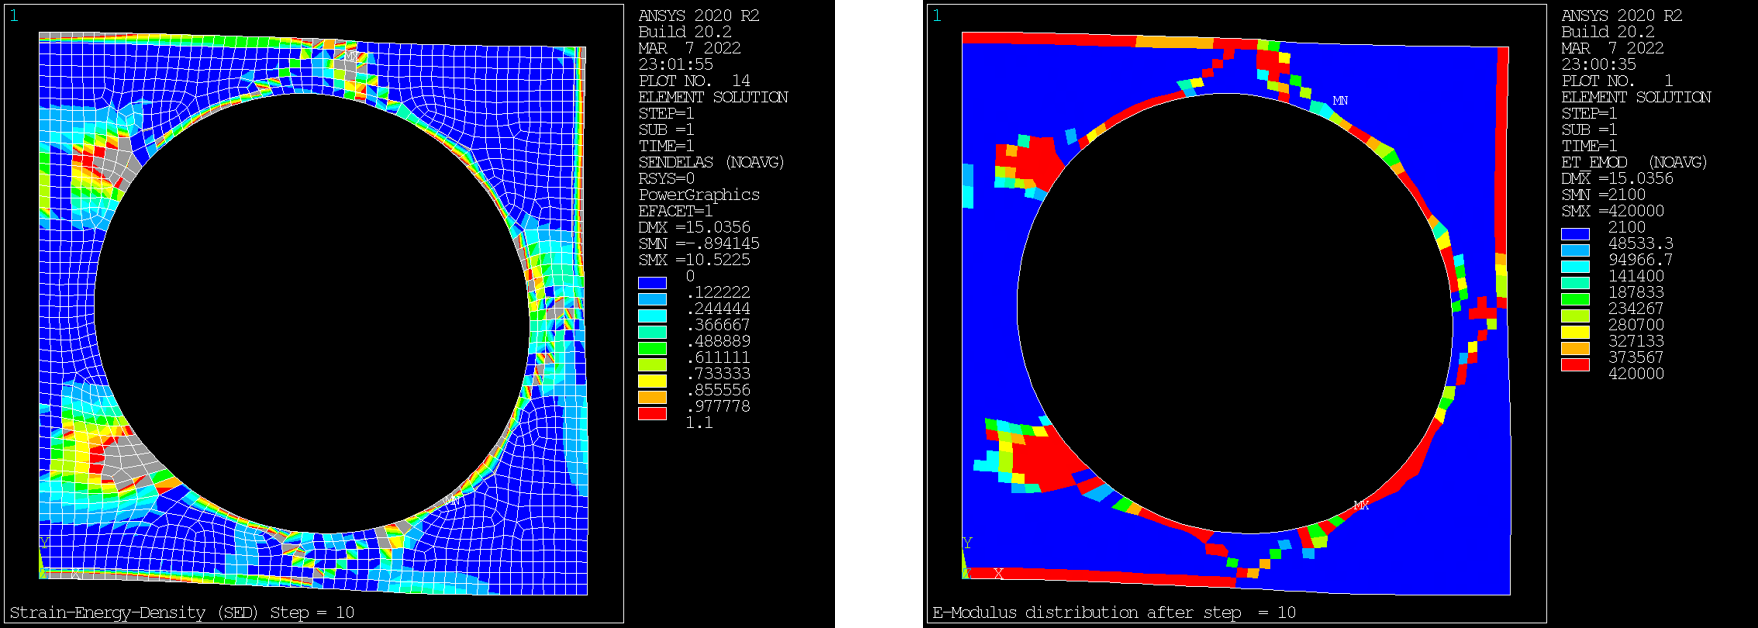
\includegraphics[width=0.9\textwidth]{pictures/2022_CW09}
	\end{figure}
	\centering Plate fixed on the left edge and with downward force on the right edge.
	Strain-Energy-Density (SED) as trigger for remodeling (left). 
	Remodeled geometry with new Young Modulus distribution (right).
\end{frame}


% ------------------------------------------------------------
% --------------------------------------------------- Slide --
\subsection{CW 10}
% ------------------------------------------------------------
% ------------------------------------------------------------
\begin{frame}
  \frametitle{Outlook CW 10}
	\begin{itemize}
		\item Continue reading in more details about bone remodeling. Start with papers from Frost, which are cited by many other researchers.
		\item Create own APDL script for Bone Remodeling. Consider a simplified geometry of bone and implant with a single material.
	\end{itemize}
\end{frame}
% --------------------------------------------------- Slide --


	%% ------------------------------------------------------------
\section{Calendar Week}
% ------------------------------------------------------------
% --------------------------------------------------- Slide --
\subsection{CW 10+11}
% ------------------------------------------------------------
\begin{frame}
  \frametitle{Review CW 10+11}
	\begin{itemize}
		\item Read papers Weinans1992, Mullender1994 and Lian2010 about bone remodeling algorithms (see attachment to email). Example of a plate representing simplified trabecular bone is shown in all 3 papers with results. We tried to reproduce these results with our own work. \textcolor{green}{Done}
		\item New APDL Script written, based on the one used for exercises provided by Uni Ulm. \textcolor{green}{Done}
		\item A lot of work to get the first results right. But now there is a fair agreement between our results and the results presented in the paper Weinans1992. \textcolor{green}{Done}
	\end{itemize}
\end{frame}

\begin{frame}
  \frametitle{Review CW 10+11 - Reproduction of Literature Results}
	\begin{figure}
		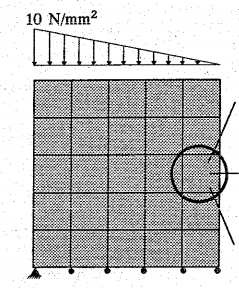
\includegraphics[width=0.3\textwidth]{pictures/2022_CW10+11_1}
	\end{figure}
	\centering Square plate representing "simplified trabecular bone" for study purposes of remodeling algorithm. 
	
	\centering Linear varying load on top edge, fixed support on bottom left corner, frictionless support on bottom edge. 
\end{frame}

\begin{frame}
  \frametitle{Review CW 10+11 - Reproduction of Literature Results}
	\begin{figure}
		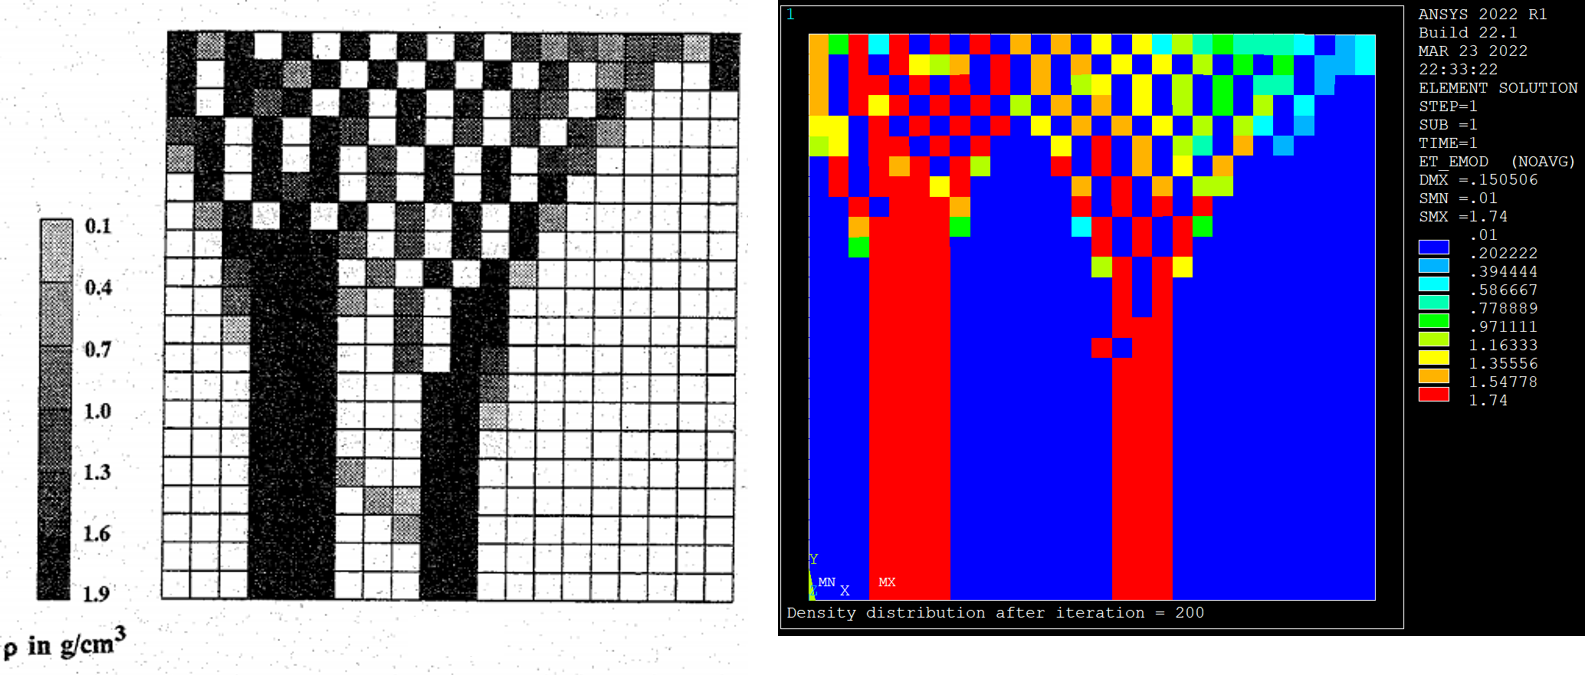
\includegraphics[width=0.9\textwidth]{pictures/2022_CW10+11_2}
	\end{figure}
	\centering Density distribution after remodeling. 
	
	\centering Results presented in the literature (left, from Weinans1992).
	
	\centering Results obtained in this work implementing equivalent algorithm with same parameters and similar mesh as in Weinans1992 (right).
\end{frame}

% ------------------------------------------------------------
% --------------------------------------------------- Slide --
\subsection{CW 12}
% ------------------------------------------------------------
% ------------------------------------------------------------
\begin{frame}
  \frametitle{Outlook CW 12}
	\begin{itemize}
		\item Reproduce bone remodeling algorithm of the other two papers mentioned in the first slide (Mullender1994 and Lian2010), which can be considered as evolution of the Weinans1992 algorithm. This should allow to get rid of the checker-board issue shown in the results of the previous slide.
		\item Further development of own APDL script for bone remodeling. Consider a simplified geometry of bone and implant with a single material.
	\end{itemize}
\end{frame}
% --------------------------------------------------- Slide --


	%% ------------------------------------------------------------
\section{Calendar Week}
% ------------------------------------------------------------
% --------------------------------------------------- Slide --
\subsection{CW 12}
% ------------------------------------------------------------
\begin{frame}
  \frametitle{Review CW 12}
	\begin{itemize}
		\item Work on reproducing further remodeling algorithms to reduce checker-board issue (see CW 10+11). New script still not working correctly. \textcolor{yellow}{In-Work}
		\item Further chapter of Misch's book finished (Ch. 11 about bone density. Important for remodeling algorithms) \textcolor{green}{Done}
	\end{itemize}
\end{frame}

% ------------------------------------------------------------
% --------------------------------------------------- Slide --
\subsection{CW 13}
% ------------------------------------------------------------
% ------------------------------------------------------------
\begin{frame}
  \frametitle{Outlook CW 13}
	\begin{itemize}
		\item Reproduce bone remodeling algorithm of the other two papers mentioned in the first slide (Mullender1994 and Lian2010), which can be considered as evolution of the Weinans1992 algorithm. This should allow to get rid of the checker-board issue shown in the results of the previous slide.
		\item Further development of own APDL script for bone remodeling. Consider a simplified geometry of bone and implant with a single material.
	\end{itemize}
\end{frame}
% --------------------------------------------------- Slide --


	% ------------------------------------------------------------
\section{Calendar Week}
% ------------------------------------------------------------
% --------------------------------------------------- Slide --
\subsection{CW 13+14}
% ------------------------------------------------------------
\begin{frame}
  \frametitle{Review CW 13+14}
	\begin{itemize}
		\item Started transferring code from standard APDL to Python API for Ansys using the pyAnsys project (see \url{https://mapdldocs.pyansys.com/}, official open-source project supported by Ansys, no extra license needed). Reason: allow to have a better readable and maintainable code in Python instead of APDL, but still have acess to all APDL functions. See a first source code example in attachment to email.  \textcolor{yellow}{In-Work}
		\item First positive results for new script using alternative algorithms. \textcolor{yellow}{In-Work}
	\end{itemize}
\end{frame}

% ------------------------------------------------------------
% --------------------------------------------------- Slide --
\subsection{CW 15}
% ------------------------------------------------------------
% ------------------------------------------------------------
\begin{frame}
  \frametitle{Outlook CW 15}
	\begin{itemize}
		\item Reproduce bone remodeling algorithm of the other two papers mentioned in the first slide (Mullender1994 and Lian2010), which can be considered as evolution of the Weinans1992 algorithm. This should allow to get rid of the checker-board issue shown in the results of the previous slide.
		\item Further development of own pyAnsys/APDL script for bone remodeling. Consider a simplified geometry of bone and implant with a single material.
	\end{itemize}
\end{frame}
% --------------------------------------------------- Slide --


\end{document}
